% !TEX TS-program = xelatex
% !TEX encoding = UTF-8 Unicode

\providecommand{\home}{../..}
\documentclass[\home/main.tex]{subfiles}

\begin{document}

% Dit hoort volgens mij eerder thuis in introductie:
%For example, a recent cloth folding pipeline by~\citeauthor{Doumanoglou2016} starts with a visual perception to detect candidate grasp points. These grasp points are then given to a planning module to move the robot end-effector to the desired position and orientation. This divide-and-conquer methodology leads to a loss of information between the different stages, resulting in the accumulation of errors. \Citeauthor{Doumanoglou2016} report difficulties when folding towels because the perception system labels them as shirts. These individual components are built in a laboratory environment with certain assumptions which are likely to be violated in an unstructured, complex environment. Inaccurate sensor readings together with deformation of the robot’s links also deteriorate the accuracy of these systems. In contrast, modern deep learning approaches try to achieve the same outcome in an end-to-end fashion. This is done by 

\chapter{Introduction}\label{ch:introduction}

\todo{Stefanie moet dit 100 procent kunnen begrijpen}

\textbf{\large{Ik ben nog volop aan het brainstormen, er zit hieronder nog geen structuur in. Dit heeft nog niet zoveel zin om na te lezen.}}

Wat is de hook van waar je vertrekt: vouwen? of meer algemene robottaken: robotbutler, dagdagelijkse taken.

Industry, household kader.
WAt soort robots hebben we, wat soort AI technieken. 
Folding uitleggen. 

We willen komen naar 
    NOOD schetsen, probleemstelling
    en zo naar research objectives. 


SOTA structuur volgen. Steeds luchtig, informeel en gradueel naar formeel.

Research contributions koppelen aan hoofdstukken. 

Op einde publicatielijst. 

\textbf{Indien vertrekken van de vouwtaak:}
A patent in $1691$ heralded a change for millions of individuals unprivileged to having a team dedicated for householding; the first washing machine. Instead of beating up clothing on rocks and blasting dirt away in quick current of local streams, one can now push clothing in to a washing machine and let it do the hard work. Yet, today the cloth laundry process is still a burden for many people around the globe. 
    bron: Mothers and Daughters of Invention: Notes for a Revised History of Technology, Autumn Stanley, Rutgers University Press, 1995, p. 301

\section{Robotic laundry}
Structuur:
\begin{itemize}
    \item Droom van robot automatisatie
    \item Robotic laundry, een voorbeeld van household taak maar ook relevant voor Vlaamse industrie en breder: vervormbare objecten
    \item Traditionele robotic pipelines: hoe + waar ze falen
    \item Moderne robotic pipelines: wat ze oplossen maar waar we nog tekort schieten (single focus op rigide objecten, grote datasets of veel exp nodig en reward hacking).
    \item Insert figure~\ref{fig:intro_end2end} maar hermaak in tikz!
\end{itemize}

Process of doing robotic laundry is visualized in Figure~\ref{fig:intro_robotic_laundry}.

\begin{figure}[htbp]
    \centering
	\subfile{figures/robotic-laundry-flow.tex}
    \caption[Task flow for robotic laundry.]{\textbf{Task flow for robotic laundry.} Figure adapted from~\autocite{Hamajima1996}.}
    \label{fig:intro_robotic_laundry}
\end{figure}

\paragraph{Why is robotic grasping difficult?}
Environment: distractions, occlusions.
Object side: material, mass, shape
Robotside: Noisy sensors, inaccurate and deteriorating robot hardware.
Classic perception systems: make strong assumptions about avialibility of data. 


\paragraph{Why is deformable object manipulation hard?}
Object rigidity is a common assumption in robotic grasping and manipulation. When programming a robot to grasp a \emph{glass} of water, one preferably exerts a large pinching force on the glass to make sure the robot does not drop the glass in the process. In this situation, it is safe to assume the glass will not deform. However, when using the same instructions to grasp a \emph{cup} of water, the cup will deform upon force interaction. This deformation might make the object slip, or even damage the cup, leading to a failed grasp.

Objects that deform are all around us: from squeezable ducks in the water tub to cables in industrial assembly factories. Consequently, there is a large category of deformable object manipulation tasks: fruit harvesting and processing, elderly dressing assistance, cable assembly, recycling plastic, and the task we embrace in this dissertation; cloth folding.

\begin{figure}
    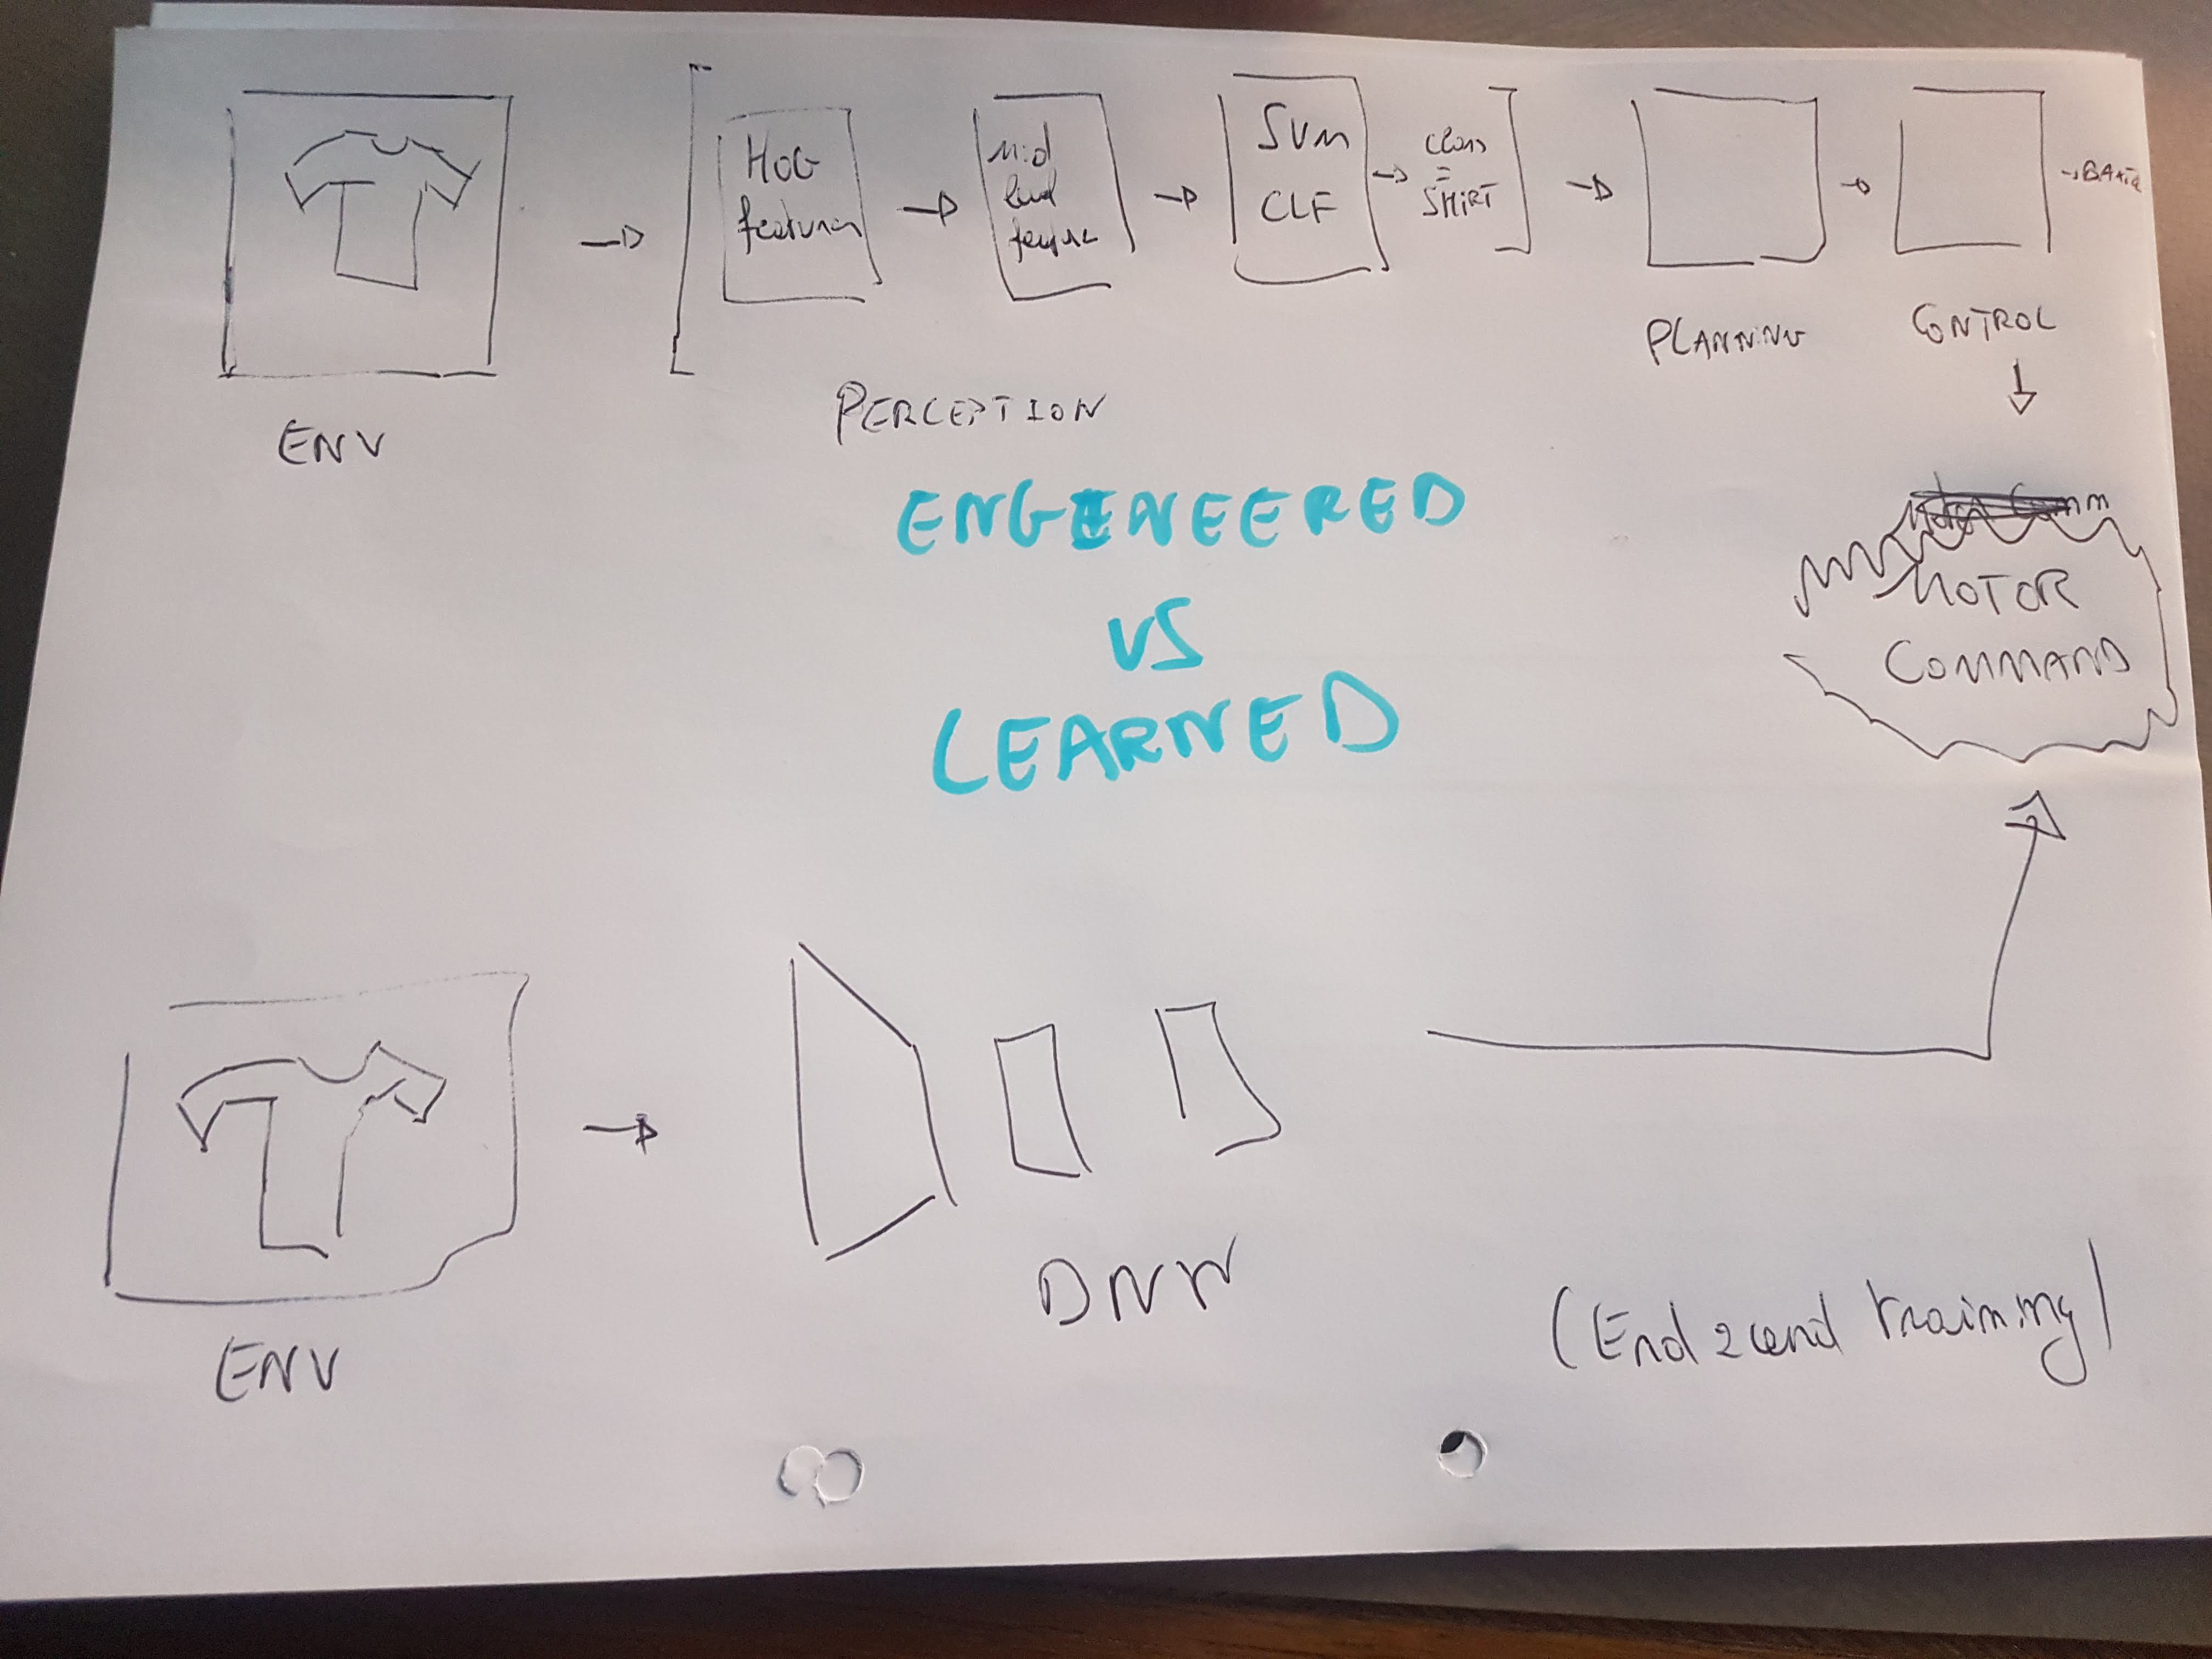
\includegraphics[width=\linewidth]{\home/chapters/01-introduction/figures/end2end-mockup}
    \caption{\textbf{Standard robotic control pipelines versus end-to-end architectures.} The diagram on the top shows how an image is processed to manually tuned features in order to do state estimation. This is then used downstream for trajectory planning and motor control. The diagram on the bottom shows an end-to-end approach to the same problem: an image is given to a deep neural network that learns its own features and executes actions directly on the actuators.}
    \label{fig:intro_end2end}
\end{figure}

\section{Robotic learning}
Machine learning introduction:
    - positioning ML %(cfr https://www.cs.cmu.edu/~tom/pubs/MachineLearning.pdf)
    - success applications: ML is preferred approach for MLP, speech recognition and computer vision , ... 
    - What is ML fundamentally. Definition. What does ML hopes to achieve ultimately? 
    - What is holding ML back in robotics? 
        Datasets, sample-efficient learning, weak or undefined learning signals 
        * a note on hardware debt.
    % - DL History    %(zie [2017[Deep learning in robotics: a review of recent research)
    %     * Linear regression has paved the way 
    %     * Activation functions allowed LR to deal with nonlinearities. Introduces biological similarities. 
    %     * Stacking layers of nonlinear models and find a way to train them
    %     * Robotics jumped on this in the 1980s.
    %     * GPUs came along for training together with large datasets. 


% \begin{figure}[htpb] 
%     \centering
% 	\subfile{\home/chapters/01-introduction/figures/ml-flow.tex}
%     \caption{\textbf{ML flow.}}
%     \label{fig:intro_ml_flow}
% \end{figure}

Self-supervised dollar bill inspiration from Epstein in 2016.


% About the positioning of this dissertation:
% \begin{figure}[htbp!]
%     \centering
%     

% Define shapes 
\def\AI_ellipse{(0, 0) ellipse [x radius=6cm, y radius=9cm, rotate=0]}
\def\ML_ellipse{(0, 0) ellipse [x radius=5cm, y radius=8cm, rotate=0]}
\def\RepresentationLearning_ellipse{(0, 0) ellipse [x radius=4cm, y radius=7cm, rotate=0]}
\def\SL_circle{(-2.0,-2.5) circle(1.5cm)}
\def\UL_circle{(2.0,-2.5) circle(1.5cm)}
\def\DL_circle{(0,0) circle(3.0cm)}
\def\RL_circle{(0, 3) circle(2.0cm)}

\begin{tikzpicture}[set/.style={fill=white,fill opacity=0.1}]

    % Help grid
    % \draw[black!5,step=0.5] (-9,-9) grid (9,9);
    % \foreach \i in {-9,-8,...,8,9}
    %     {
    %         \node[below] at (\i,-9){\small \i};
    %         \node[left] at (-9,\i){\small \i};
    %     }

    % Draw ellipses
    \draw \AI_ellipse node [label={[xshift=0.0cm, yshift=-8.75cm]Artificial intelligence}] {};
    \draw \ML_ellipse node [label={[xshift=0.0cm, yshift=-7.75cm]Machine learning}] {};
    \draw \RepresentationLearning_ellipse node [label={[xshift=0.0cm, yshift=-6.5cm,align=center]Representation\\learning}] {};

    % Color Intersection of DL and RL 
    \begin{scope}
        \clip \DL_circle;
        \clip \RL_circle;
        \fill[orange!60](0,0) circle(3cm);
    \end{scope}

    % Draw labels
    \node[set,label={Deep learning}] (DL) at (0,-0.5) {};
    \node[set,label={[align=center]Supervised\\learning}] (SL) at (-2.15,-4.0) {};
    \node[set,label={[align=center]Unsupervised\\learning}] (UL) at (2.0,-4.0) {};
    \node[set,label={[align=center]Reinforcement\\learning}] (RL) at (0, 3) {};
    \node[set,label={[align=center]Deep reinforcement\\learning}] at (barycentric cs:RL=1,DL=1) {};

    % Draw circles
    \draw \SL_circle;
    \draw \UL_circle;
    \draw \DL_circle;
    \draw \RL_circle;

\end{tikzpicture}
%     \caption{\textbf{Positioning of this research within AI domain.}}
%     \label{fig:venn_positioning_thesis}
% \end{figure}

% Focus within \gls{DRL} in this dissertation:
% \begin{figure}[htb]
%     \centering
%         \subfile{figures/RL-loop}
%     \caption{\textbf{Positioning of this research within DRL domain.}}
%     \label{fig:RL_loop_positioning}
% \end{figure}

% Focus application within robotics in this dissertation:
% \begin{figure}[htb]
%     \centering
%         \subfile{figures/positioning-application-domain}
%     \caption{\textbf{Positioning of the application domain of this research within robotics domain.}}
%     \label{fig:RL_loop_positioning}
% \end{figure}

\section{Accelerating robotic learning}
\subsection{Datasets}
\subsection{Simulation}
\subsection{Instrumentation}
When we use our hands to crush a plastic cup, multiple sensors of our body activates: we use our eyes to observe the deformations, our ears register the amplitude of the impact, our hands notify us of how much force we are applying and our proprioceptive system signal us how much crumbling there still can be done. This rich interplay of multiple modalities in the human cognitive system is in stark contrast to robotic manipulation pipelines that are largely vision-based.  Vision is important for robotic manipulation: it helps inferring the object location relative to the robot end-effectors, it helps understanding the objects geometry and some of its physical properties. Furthermore, commercial cameras are readily available and accessible compared to other sensors such as tactile sensors. Nevertheless, considering the giant leaps of object recognition using deep learning, robots still struggle recognizing objects in more difficult contexts such as partial occlusion, transparent object and moving objects \autocite{Guo2014,sajjan2019cleargrasp,Ojha2015}. 
Incorporating heterogenous sources of information can alleviate problems when state estimation cannot be directly observed from pixels. For example, finding the occluded corner of a crumbled towel is possible using sensing and simplifies the folding process considerably. 
We denote the process of adding sensory information to the learning environment of a robot as \textbf{instrumentation}. The goal is to direct the large focus on using vision-based state estimation to applying other sensor modalities in the environment such as tactile sensing in a cloth and force sensing in the fingers. Our hypothesis is that some modalities encode parts of the state in a much compacter way compared to vision. This semantic more meaningful encoding accelerates learning, which is important in robotics where real rollouts are expensive. 

% losse gedachten, geen zinnen:
%     het is dus een combinatie van 
%         robot instrumentation = multi-modal learning: cameras, tactile sensors, force sensors op de robot 
%         env instrumentation = example, place a scale to weight the object 
%         object instrumentation = smart cloth 

\section{From behavioral cloning to understanding task intent}
\section{Research contributions} \label{sec:intro_contributions}
\begin{itemize}
    \item Dataset with people folding clothing
    \item Unsupervised reward function
    \item Low-cost robot setup to fold cloth invivo
    \item Instrumentation
    \item Gripper for folding
\end{itemize}

\section{Thesis structure}
This thesis is structured to first provide preliminary background and a review of the relevant literature. The remainder of the thesis deals with the methodology and results iterated in the previous Section~\ref{sec:intro_contributions}. The structure is as follows:
\begin{itemize}
    \item In Chapter~\ref{ch:lit}, we
\end{itemize}


\end{document}
